\chapter{\Vauc as a toolkit}

\Vauc provides several programs that manipulate various types of
automata. In this chapter we will learn how to use those
programs. Actually there are 6 programs located in
src/demos/function\_library/ directory. Each of them dealing with a
specific type of automata:
\begin{description}
  \item [b] for manipulating automata over Boolean semiring $\mathbb{B}$;
  \item [z] for manipulating automata over $(\mathbb{Z},+)$;
  \item [z\_min\_plus] for manipulating automata over $(\mathbb{Z},min)$;
  \item [z\_max\_plus] for manipulating automata over $(\mathbb{Z},max)$;
  \item [rt\_tdc] for manipulating realtime transducers;
  \item [tdc] for manipulating automata over free monoid product.
\end{description}
The first step before starting to work with \Vauc toolkit is to choose
on which type of automata you intend to work. Then you should just use
the proper program between those listed before.

All automata used in this chapter can be found in the
\textbf{doc/manual/examples/} directory.
\newpage

%%Example on Boolean automaton
\section{Boolean automata}

This part shows the use of the program \textit{b}.

\subsection{A first example}

Let's consider the following Boolean automaton \autoref{A_1}.
%%Schema de l'automate A1
\begin{figure}[ht] \centering
  \begin{VCPicture}{(0,-2)(6,2)}
    % states
    \State{(0,0)}{A} \State{(3,0)}{B} \State{(6,0)}{C}
    % initial--final
    \Initial{A} \Final{C}
    % transitions
    \EdgeL{A}{B}{a} \EdgeL{B}{C}{b}
    \LoopS[.5]{A}{b} \LoopN[.5]{A}{a} \LoopS[.5]{C}{b} \LoopN[.5]{C}{a}
    %
  \end{VCPicture}
  \caption{The automaton $A_1$}
  \label{A_1}
\end{figure}
We will use \Vauc to compute the determinized automaton of $A_1$ and
then we will minimize the resulting automaton.

\subsubsection{Determinization of $A_1$}
Computing the determinized of a Boolean automaton is simply realized
by calling \textit{determinize} function:
\begin{alltt}
# ./b determinize a1.xml > a1\_det.xml
\end{alltt}
Now the file a1\_det.xml contains the XML description of the
determinized of the automaton A.

\subsubsection{Visualizing}

We can get some information about our newly created automaton by calling
the \textit{info} function:
\begin{alltt}
# ./b info a1\_det.xml
\textit{States: 4
Transitions: 8
Initial states: 1
Final states: 2}
\end{alltt}
Or we can use dotty to visualize our newly created automaton:
\begin{alltt}
# ./b display a1\_det.xml
\end{alltt}

%%Dotty output of det(A1)
%%\begin{figure}[ht]
\begin{center}
  \scalebox{0.7}{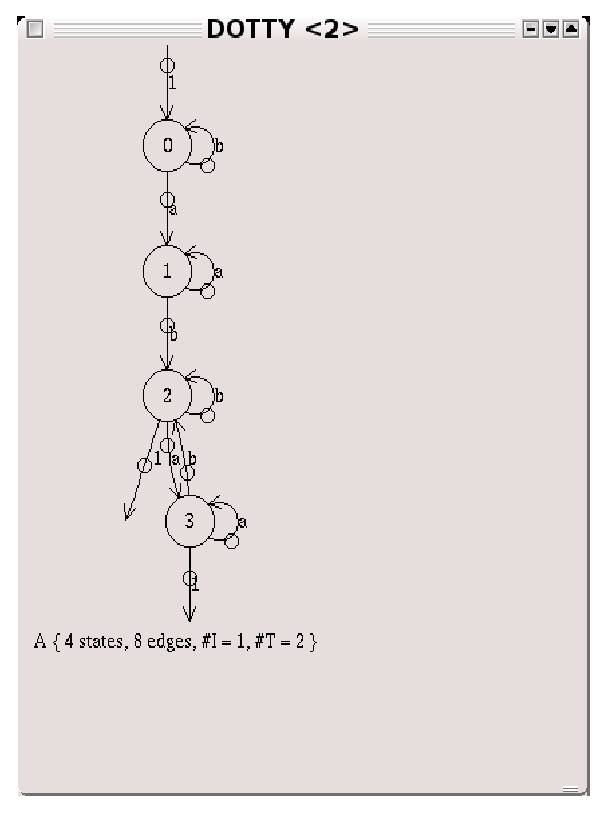
\includegraphics{images/a1_det.eps}}
\end{center}
%%  \caption{Determinized of $A_1$}
%%\end{figure}

\subsubsection{Minimizing}

\begin{alltt}
# ./b determinize a1.xml | ./b minimize - | ./b display -
\end{alltt}

%% Dotty min(det(A1))
%%\begin{figure}[!h]
\begin{center}
  \scalebox{0.7}{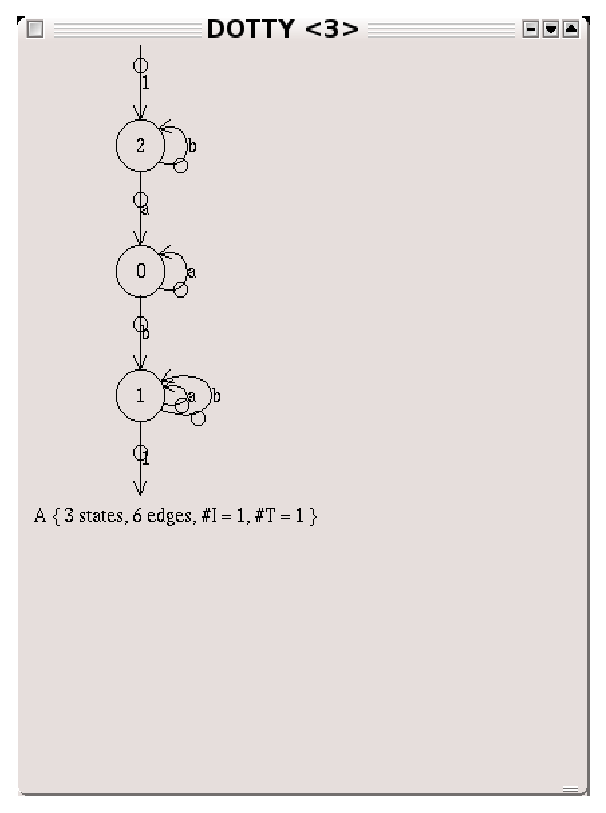
\includegraphics{images/a1_det_min.eps}}
\end{center}
%%\caption{Minimizing the Determinized of $A_1$}
%%\end{figure}

\subsubsection{Evaluation}

Evaluating if a word is accepted by our automaton:
\begin{alltt}
# ./b eval a1.xml 'abab'
\textit{1}
# ./b eval a1.xml 'bbba'
\textit{0}
\end{alltt}
where 1 (resp. 0) means that the word is accepted (resp. not accepted)
by the automaton.

\subsection{Rational expressions and Boolean automata}

\Vauc provides functions for manipulating rational expressions
associated to Boolean automata. For instance, computing the language
recognized by a Boolean automaton can be done thanks to the
\textit{aut\_to\_exp} function:
\begin{alltt}
# ./b aut_to_exp a1.xml
\textit{(a+b)*.a.b.(a+b)*}
# ./b aut_to_exp a1_det.xml
\textit{b*.a.a*.b.(a.a*.b+b)*.(a.a*+1)}
\end{alltt}
Plus \Vauc provides several algorithms that build an automaton that
recognizes a given language. For instance let's build the standard
automaton that recognizes the language "$(a+b)*a.b.(a+b)*$" and
minimize the resulting automaton:

\begin{alltt}
# /b standard_of "(a+b)*a.b.(a+b)*" | ./b minimize - | ./b display -
\end{alltt}
%%\begin{figure}[ht]
\begin{center}
  \scalebox{0.7}{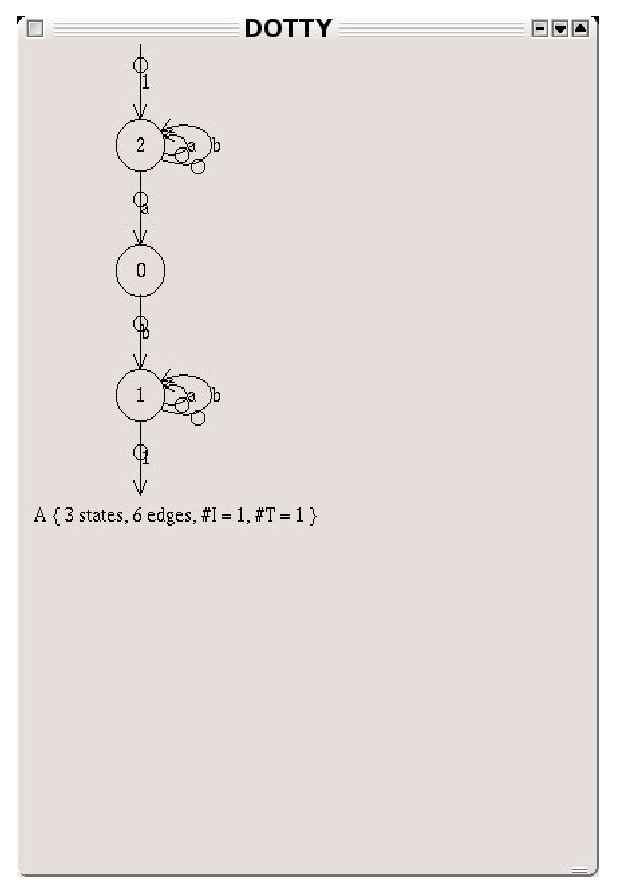
\includegraphics{images/a1.eps}}
\end{center}
%%  \caption{The minimize standard automaton of "(a+b)*a.b.(a+b)*"}
%%\end{figure}
%%Please note that your rational expressions should follow the
%%following grammar. %%Fixme : Lien vers la grammaire des ratexp

\subsection{Available functions}
%% Une definition plus rigoureuse des algorithmes devrait etre fournie
%% en annexe.
In this section you will find a brief definition of all functions that
\Vauc provides for manipulating Boolean automata.
\begin{itemize}
\item a1.xml and a2.xml are two Boolean automata described in
  \Vauc XML format.
\item w is a word, for example \textit{"aabb"} if you are working on an
  alphabet that contains the letters \textit{a} and \textit{b}.
\item exp is a rational expression denoting a language.
\item n is a strictly positive integer.
\end{itemize}

\begin{description}
  \item [are-isomorphic]
    ./b a1.xml a2.xml\\
    Return 1 (resp. 0) if the two automata are (resp. aren't)
    isomorphic.

  \item [aut\_to\_exp]
    ./b aut\_to\_exp a1.xml\\
    Return a regular expression denoting the language recognized by
    \textit{aut}.

  \item [accessible]
    ./b accessible a1.xml\\
    Extract the sub-automaton of accessible states of a1.xml.

  \item [closure]
    ./b closure a1.xml\\
    Complete the automaton a1.xml to make it
    closed over epsilon transition (based on the
    Floyd-McNaughton-Yamada algorithm).

  \item [co-accessible]
    ./b accessible a1.xml\\
    Extract the sub-automaton of co-accessible states of a1.xml.

  \item [derived\_terms]
    ./b derived\_terms exp\\
    Return the Boolean automaton build from the derived terms of exp.

  \item [determinize]
    ./b determinize a1.xml\\
    Return the determinized of a1.xml.

  \item [display]
    ./b display a1.xml\\
    Display a graphical view of the automaton a1.xml using DOT format.

  \item [evaluation]
    ./b eval a1.xml w\\
    Return 1 (resp. 0) if the word w is accepted by the automaton
    a1.xml

  \item [expand]
    ./b expand exp\\
    Return the expanded expression of exp.

  \item [info]
    ./b info a1.xml\\
    Display general information (Number of states, number of
    transitions, number of initial states and number of final
    states) on the automaton \textit{a1.xml}.

  \item [is-empty]
    ./b is-empty a1.xml\\
    Return 1 (resp. 0) if the automaton has (resp. hasn't) accessible
    or (resp. and) co-accessible states.

  \item [minimize]
    ./b minimize [hm] a1.xml\\
    Return the minimal automaton of a1.xml (By default the minimal
    automaton is built using Hopcroft algorithm).
    \begin{description}
      \item [h] Use Hopcroft algorithm
      \item [m] Use Moore algorithm
    \end{description}

  \item [power]
    ./b power a1.xml n\\
    Return a1.xml to the power of n.

  \item [product]
    ./b product a1.xml a2.xml\\
    Return the product of the two automata.

  \item [quotient]
    ./b quotient a1.xml\\
    Return the quotient of a non deterministic automaton.

  \item [realtime]
    ./b realtime a1.xml\\
    Return the realtime automaton of the automaton a1.xml.

  \item [standard\_of]
    ./b standard\_of exp\\
    Return the standard automaton build from the rational expression exp.

  \item [transpose]
    ./b transpose a1.xml\\
    Return the transposed of the automaton a1.xml.

  \item [trim]
    ./b trim a1.xml\\
    Return the trimmed automaton of a1.xml.

  \item [thompson\_of]
    ./b thompson\_of exp\\
    Return the Thompson automaton of the rational expression exp.
\end{description}
\newpage

\section{Transducers}

This section deals with transducers. In \Vauc we distinguish two types
of transducers. The first one is considering a transducer as a
weighted automaton of a product of free monoid (the \textbf{tdc}
program). The second one is considering a transducer as a machine that
takes a word as input and produce another word as output (the
\textbf{rt\_tdc}). One can consider that both views are equivalent and
\Vauc actually provides algorithms to pass from a view to the other one.

\subsection{Example}

The transducer $T_1$(\autoref{bindiv3}) gives the quotient by 3 of a
binary number and the transducer $T_2$(\autoref{add1}) adds 1 to a binary number.

\begin{figure}[h]
  \begin{center}
    \begin{VCPicture}{(0,-2)(6,2)}
% states
\State{(0,0)}{A} \State{(3,0)}{B} \State{(6,0)}{C}
\Initial[w]{A}
\Final[s]{A}
%transitions
\LoopN[.5]{A}{\IOL{a}{a}}
\LoopN[.5]{C}{\IOL{b}{b}}
\ArcL{A}{B}{\IOL{b}{a}}
\ArcL{B}{A}{\IOL{b}{b}}
\ArcL{B}{C}{\IOL{a}{a}}
\ArcL{C}{B}{\IOL{a}{b}}
\end{VCPicture}
\caption{Transducer $T_1$ computing the quotient by 3 of a binary number}
\label{bindiv3}
  \end{center}
\end{figure}
\begin{figure}[h]
  \begin{center}
    \begin{VCPicture}{(0,-2)(3,2)}
% states
\State{(0,0)}{A} \State{(3,0)}{B}
\Initial[w]{A}
\FinalL{s}{A}{\IOL{}{b}}
\Final[e]{B}
%transitions
\LoopN[.5]{A}{\IOL{b}{a}}
\LoopN[.5]{B}{\IOL{b}{b}}
\LoopS[.5]{B}{\IOL{a}{a}}
\EdgeL{A}{B}{\IOL{a}{b}}
\end{VCPicture}
\caption{Transducer $T_2$ adding 1 to a binary number}
\label{add1}
  \end{center}
\end{figure}

\subsubsection{Evaluation}
\begin{alltt}
# ./rt_tdc evaluation quot_3_rt.xml 'bba'
\textit{a.b.a}
\end{alltt}

\subsubsection{Domain}
The transducer $T$ only accepts binary number which are divisible by 3
as input.
\begin{alltt}
# ./rt_tdc domain quot_3_rt.xml > divisible_by_3.xml
\end{alltt}
Now the file divisible\_by\_3.xml contains the description of a Boolean
automaton that accepts only the numbers divisible by 3.

\subsubsection{to-tdc}
Each transucers can be transformed to the other type of transducer
thanks to the ``to-tdc'' and ``to-rt-tdc'' functions.
\begin{alltt}
# ./rt_tdc to-tdc quot_3_rt.xml > quot_3.xml
# ./rt_tdc to-tdc add1_rt.xml > add1.xml
\end{alltt}

\subsubsection{Composing}
\begin{alltt}
# ./tdc compose quot_3.xml add1.xml
\end{alltt}

\subsection{Available functions}

\begin{itemize}
\item t1.xml and t2.xml are two transducers (either ``realtime'' or
  not) described in \Vauc XML format.
\item w is a word, for example \textit{"aabb"} if you are working on an
  alphabet that contains the letters \textit{a} and \textit{b}.
\item a.xml is a Boolean automaton.
\item t1\_rt.xml is a realtime transducer.
\item t1\_fmp.xml is a transducer (seen as an automaton over a free monoid
  product).
\end{itemize}
The following functions are available for both rt\_tdc and tdc program:
\begin{description}
  \item [are-isomorphic]
    ./tdc t1.xml t2.xml\\
    Return 1 (resp. 0) if the two transducers are (resp. aren't)
    isomorphic.

  \item [closure]
    ./tdc closure t1.xml\\
    Complete the transducer t1.xml to make it
    closed over epsilon transition (based on the
    Floyd-McNaughton-Yamada algorithm).

  \item [compose]
    ./tdc compose t1.xml t2.xml\\
    Return the composed transducer from t1.xml and t2.xml. t1.xml and
    t2.xml must be the same type of transducers.

  \item [display]
    ./tdc display t1.xml\\
    Display a graphical view of the transducer t1.xml using DOT format.

  \item [domain]
    ./tdc domain t1.xml\\
    Return an automaton describing all input accepted by the
    transducer t1.xml.

  \item [evaluation]
    ./tdc evaluation t1.xml w\\
    Return the evaluation of w by t1.xml.

  \item [evaluation\_aut]
    ./tdc evaluation\_aut t1.xml a.xml\\
    Return a Boolean automaton describing the words produced by the
    language described by a.xml evaluated by t1.xml.

  \item [image]
    ./tdc image t1.xml\\
    Return an automaton describing all output produced by the
    transducer t1.xml.

  \item [info]
    ./tdc info t1.xml\\
    Display general information (Number of states, number of
    transitions, number of initial states and number of final
    states) on the transducer \textit{t1.xml}.

  \item [is-empty]
    ./tdc is-empty t1.xml\\
    Return 1 (resp. 0) if the transducer has (resp. hasn't) accessible
    or (resp. and) co-accessible states.

  \item [transpose]
    ./tdc transpose t1.xml\\
    Return the transposed of the transducer t1.xml.

  \item [trim]
    ./tdc trim t1.xml\\
    Return the trimmed transducer of t1.xml.
\end{description}

\subsubsection{Algorithms for ``realtime'' transducers}

\begin{description}
%%Fixme: ambigue
\item [realtime]
./rt\_tdc realtime t1\_rt.xml\\
Return the realtime transducer of t1\_rt.xml.

\item [is-realtime]
./rt\_tdc is-realtime t1\_rt.xml\\
Return 1 (resp. 0) if the transducer t1\_rt.xml is (isn't) realtime.

\item [to-tdc]
./rt\_tdc to-tdc t1\_rt.xml\\
Return the equivalent fmp transducer of t1\_rt.xml.
\end{description}

\subsubsection{Algorithms for transducers}
%%Fixme : A finir
\begin{description}
\item [sub-normalize]
  ./tdc sub-normalize t1\_fmp.xml\\
  Return the sub-normalized transducer of t1\_fmp.xml.

\item [is-sub-normalized]
  ./tdc is-sub-normalized t1\_fmp.xml
  Return 1 (resp. 0) if the t1\_fmp.xml is (isn't) sub-normalized.

\item [composition-cover]
  ./tdc composition-cover t1\_fmp.xml

\item [composition-co-cover]
  ./tdc composition-co-cover t1\_fmp.xml

\item [b-compose]
  ./tdc b-compose t1\_fmp.xml t2\_fmp.xml

\item [to-rt-tdc]
  ./tdc to-rt-tdc t1\_fmp.xml\\
  Return the equivalent realtime transducer of t1\_fmp.xml.

\item [intersection]
  ./tdc intersection t1\_fmp.xml

\end{description}
\newpage

\section{Weighted automata}

This part shows the use of the program \textit{z}, but all
comments should also stand for the programs \textit{z\_min\_plus and
z\_max\_plus}.

\subsection{Example}

Let's consider the following $\mathbb{N}$-automaton, \textit{i.e.}
an automaton which label's weights are in $\mathbb{N}$:

%%Schema de l'automate B1
\begin{figure}[ht] \centering
  \begin{VCPicture}{(0,-2)(3,2)}
    % states
    \State{(0,0)}{A} \State{(3,0)}{B}
    % initial--final
    \Initial{A} \Final{B}
    % transitions
    \EdgeL{A}{B}{b}
    \LoopS[.5]{A}{b} \LoopN[.5]{A}{a}
    \LoopS[.5]{B}{b} \LoopN[.5]{B}{a}
    %
  \end{VCPicture}
  \caption{The automaton $B_1$}
\end{figure}

This time the evaluation of the word \textit{w} by the automaton $B_1$
will produce a number, rather than simply accept or reject \textit{w}.
For instance let's evaluate "abab" and "bbab":

\subsubsection{Evaluation}

\begin{alltt}
# ./z eval b1.xml 'abbb'
\textit{3}
# ./z eval b1.xml 'abab'
\textit{2}
\end{alltt}

As you may have already guessed the automaton $B_1$ "counts" the
number of 'b' contained in \textit{w}.

\subsubsection{Power}

Now let's consider the $B_1^4$, where
$$B_1^4 = \prod_{i=1}^4 B_1, 4 > 0$$

\begin{alltt}
# ./z power b1.xml 4 > b1_4.xml
\end{alltt}

Now the file \textit{b1\_4.xml} contains the automaton $B_1^4$. Lets
see what the evaluation of the words "abab" and "bbab" gives with this
automaton:

\begin{alltt}
#./z eval b1_4.xml 'bbab'
\textit{81}
./z eval b1_4.xml 'abab'
\textit{16}
\end{alltt}

This time one can notice that the automaton $B_1^4$ returns the
evaluation of $B_1$ at power 4.

\subsubsection{quotient}

One drawback of doing successive products of an automaton is
that it creates a lot of new states and transitions.
\begin{alltt}
#./z power b1.xml 4 | ./z info -
\textit{States: 16}
\textit{Transitions: 97}
\textit{Initial states: 1}
\textit{Final states: 1}
\end{alltt}
One way of reducing the size of our automaton is to use the "quotient"
algorithm.
\begin{alltt}
#./z power b1.xml 4 | ./z quotient - | ./z info -
\textit{States: 5}
\textit{Transitions: 15}
\textit{Initial states: 1}
\textit{Final states: 1}
\end{alltt}

\subsection{Available functions}
In this section you will find a brief definition of all functions for
manipulating weighted automata.
\begin{itemize}
\item a1.xml and a2.xml are two weighted automata described in
  \Vauc XML format.
\item w is a word, for example \textit{"aabb"} if you are working on an
  alphabet that contains the letters \textit{a} and \textit{b}.
\item exp is a rational expression denoting a language.
\item n is a strictly positive integer.
\end{itemize}

\begin{description}
  \item [are-isomorphic]
    ./z a1.xml a2.xml\\
    Return 1 (resp. 0) if the two automata are (resp. aren't)
    isomorphic.

  \item [aut\_to\_exp]
    ./z aut\_to\_exp a1.xml\\
    %%Fixme

  \item [accessible]
    ./z accessible a1.xml\\
    Extract the sub-automaton of accessible states of a1.xml.

  \item [closure]
    ./z closure a1.xml\\
    Complete the automaton a1.xml to make it
    closed over epsilon transition (based on the
    Floyd-McNaughton-Yamada algorithm).

  \item [co-accessible]
    ./z accessible a1.xml\\
    Extract the sub-automaton of co-accessible states of a1.xml.

  \item [derived\_terms]
    ./z derived\_terms exp\\
    Return the weighted automaton build from the derived terms of exp.

  \item [determinize]
    ./z determinize a1.xml\\
    Return the determinized of a1.xml.

  \item [display]
    ./z display a1.xml\\
    Display a graphical view of the automaton a1.xml using DOT format.

  \item [evaluation]
    ./z eval a1.xml w\\
    Return the evaluation of w by a1.xml.

  \item [expand]
    ./z expand exp\\
    Return the expanded expression of exp.

  \item [info]
    ./z info a1.xml\\
    Display general information (Number of states, number of
    transitions, number of initial states and number of final
    states) on the automaton \textit{a1.xml}.

  \item [is-empty]
    ./z is-empty a1.xml\\
    Return 1 (resp. 0) if the automaton has (resp. hasn't) accessible
    or (resp. and) co-accessible states.

  \item [minimize]
    ./z minimize [hm] a1.xml\\
    Return the minimal automaton of a1.xml (By default the minimal
    automaton is built using Hopcroft algorithm).
    \begin{description}
      \item [h] Use Hopcroft algorithm
      \item [m] Use Moore algorithm
    \end{description}

  \item [power]
    ./z power a1.xml n\\
    Return a1.xml to the power of n.

  \item [product]
    ./z product a1.xml a2.xml\\
    Return the product of the two automata.

  \item [quotient]
    ./z quotient a1.xml\\
    Return the quotient of a non deterministic automaton.

  \item [realtime]
    ./z realtime a1.xml\\
    Return the realtime automaton of the automaton a1.xml.

  \item [standard\_of]
    ./z standard\_of exp\\
    Return the standard automaton build from the rational expression exp.

  \item [transpose]
    ./z transpose a1.xml\\
    Return the transposed of the automaton a1.xml.

  \item [trim]
    ./z trim a1.xml\\
    Return the trimmed automaton of a1.xml.

  \item [thompson\_of]
    ./z thompson\_of exp\\
    Return the Thompson automaton of the rational expression exp.
\end{description}
\newpage

\section{Building your own automaton}
%%FIXME: Here we should give the usage of define_automaton function.
